\cotefile{10}
\scanpage{115}
% archive sheet number: 114

Chapitre 1. Généralités sur les opérations $\otimes$ sur une catégorie.

\inserted{\handwritten{Appendice: Rappels sur les coalgèbres, comodules, bigèbres.....}}

Chapitre 2. Relations entre $\otimes$-catégories \deleted{et} avec foncteur fibre, et coalgèbres resp. hyperalgèbres: \deleted{\unsure{Group}} Dualité de Tannaka.

\hfill (structures mixtes, connexions ....)

Chapitre 3. \uline{Exemples nombreux et divers.} \uline{Dictionnaire détaillé.}

\margin{\handwritten{\figure{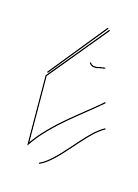
\begin{tikzpicture}[x=0.35cm,y=0.35cm]
\draw (2.9,4.8) -- (0.7,3.2);
\draw (2.95,4.72) -- (0.65,3.08) -- (0,0.6) .. controls (0.8,1.3) and (2,1.7) .. (2.8,2.1);
\draw (2.25,3.55) .. controls (2.35,3.3) and (2.55,3.4) .. (2.8,3.35);
\draw (0.4,-0.1) .. controls (1.1,0) and (2.1,1.0) .. (2.8,1.15);
\end{tikzpicture}}}}
Chapitre 4. Filtrations sur un foncteur fibre.

Chapitre 5. Théorème de structure des $\otimes$-catégories en termes de gerbes.

Chapitre 6. Polarisation d'une $\otimes$-catégorie. Groupes de Hodge.

Chapitre 7. $\otimes$-Catégories à lien réductif. Classification sur \uline{$R$}.

\unsure{8hapitre|Chapitre} 8. Structures de Hodge, groupes de Mumford-Tate et espaces modulaires correspondants.

Chapitre 9. Questions d'effectivité (?)

\handwritten{Éventuellement un chapitre de \unsure{Armature} sur le ``cas non commutatif''}

\handwritten{Un autre sur variantes pour catégories \uline{triangulées} ?}

\handwritten{Chapitre sur catégories de Picard,(plus gén.\ \unsure{gr.poïdes|g.poïdes} avec loi $\otimes$) catégories de Picard enveloppantes. Cas des catégories ayant deux loi $\oplus$ et $\otimes$ ----}
